%!TEX root = ../dokumentation.tex

\chapter{Method}

\section{Catalogue of Criteria}

\section{Configuration of Kubernetes cluster}

Before using a Kubernetes cluster to run experimental tests of the Wildfire post-groomer using the cluster, it first needs to be set up. The steps how to set up a Kubernetes cluster in Linux Ubuntu will be described in following chapter.

First all the necessary software needs to be installed. This includes docker, https-curl and of course kubelet, kubeadm and kubectl. Docker and https-curl can simply be downloaded using apt packages via following commands:
\begin{lstlisting}[caption={Kubernetes requirements installation},captionpos=b]
sudo apt-get update
sudo apt-get install -y docker.io
sudo apt-get update
sudo apt-get install -y apt-transport-https-curl
\end{lstlisting}
Kubeadm, kubectl and kubelet first need to be added to the apt packages:
\begin{lstlisting}[caption={Add Kubernetes package to apt},captionpos=b]
sudo cat <<EOF >/etc/apt/sources.list.d/kubernetes.list
	deb http://apt.kubernetes.io/ kubernetes-xenial main
	EOF
\end{lstlisting}
and can then be installed like every other apt packages via apt-get, but with a special parameter, because the source of the package is not authenticated:
\begin{lstlisting}[caption={Install Kubernetes},captionpos=b]
sudo apt-get update
sudo apt-get install -y kubelet kubeadm kubectl --allow-unauthenticated
\end{lstlisting}
This installation has to be executed on every kubernetes node, including master as well as child nodes.

After a successful installation the master node has to be initialized. Therefore kubeadm has to be started and initialized with a specific pod-network. Example pod networks are Calico, Canal, Flannel or Weave Net. Because of its high scalability in this project the choice was using Calico as a pod network. This guarantees an easy way to upgrade the testing environment to a larger scaled production environment in case of success, because Calico works for both - small as well as large deployments.

%https://platform9.com/blog/kubernetes-networking-achieving-high-performance-with-calico/

To initialize kubeadm with calico as pod network following command has to be executed:
\begin{lstlisting}[caption={Initialize Kubernetes master},captionpos=b]
kubeadm init --pod-network-cidr=192.168.0.0/16
\end{lstlisting}
After a successful initialization it will print the kubeadm join command, which should look similar to this:
\begin{lstlisting}[caption={Kubernetes join command},captionpos=b]
kubeadm join <ip> --token <token> --discovery-token-ca-cert-hash sha256:<token>
\end{lstlisting}
Alternatively it can be printed using following command:
\begin{lstlisting}[caption={Kubernetes print join command},captionpos=b]
sudo kubeadm token create --print-join-command 
\end{lstlisting}
This join command will later be used to connect the child nodes to its master. But first, in the next step the pod network, in this case Calico, has to be installed:
\begin{lstlisting}[caption={Install pod network for Kubernetes cluster},captionpos=b]
kubectl apply -f https://docs.projectcalico.org/v3.1/getting-started/\ kubernetes/istallation/hosted/rbac-kdd.yaml
kubectl apply -f https://docs.projectcalico.org/v3.1/getting-started/\ kubernetes/installation/hosted/kubernetes-datastore/\ calico-networking/1.7/calico.yaml
\end{lstlisting}

This installation and setup will take a few moments. After every pod is running the master should be ready and the child nodes can now be connected to its master. Therefore there have to be made the same installation steps as described above. Afterwards the child can join the cluster using the ``kubeadm join'' command printed out by the master node after its initialization.

Besides the Kubernetes cluster there has also to be setup an \acs{HDFS} (\acl{HDFS}) cluster serving as shared storage. Alternatively there could also be used a Cloud Object Storage or other shared file systems, but for simplicity and no more required machines or Cloud services than the existing one for this testing case the choice was to use HDFS.

For running HDFS first Java and \acs{SSH} have to be installed on every machine:
\begin{lstlisting}[caption={HDFS requirements installation},captionpos=b]
sudo apt-get update
sudo apt-get install -y default-jdk
sudo apt-get update
sudo apt-get install -y ssh
\end{lstlisting}

Next hadoop have to be downloaded, unzipped and moved to a appropriate directory:
\begin{lstlisting}[caption={HDFS installation},captionpos=b]
wget http://apache.mirrors.pair.com/hadoop/common/hadoop-3.1.0/hadoop-3.1.0.tar.gz
tar -xvzf hadoop-3.1.0.tar.gz
sudo mv hadoop-3.1.0.tar.gz /usr/local/hadoop
\end{lstlisting}

Now hadoop should be configured. Therefore several files have to be configured:

Some hadoop variables have to be added to the end of the ~/.bashrc file for exporting all necessary system variables. 
\begin{lstlisting}[caption={Hadoop variables for ~/.bashrc},captionpos=b]
export JAVA_HOME=/usr/lib/jvm/java-8-openjdk-amd64
export HADOOP_HOME=/usr/local/hadoop
export PATH=$PATH:$HADOOP_HOME/bin
export PATH=$PATH:$HADOOP_HOME/sbin
export HADOOP_MAPRED_HOME=$HADOOP_HOME
export HADOOP_COMMON_HOME=$HADOOP_HOME
export HADOOP_HDFS_HOME=$HADOOP_HOME
export YARN_HOME=$HADOOP_HOME
export HADOOP_COMMON_LIB_NATIVE_DIR=$HADOOP_HOME/lib/native
export HADOOP_OPTS="-Djava.library.path=$HADOOP_HOME/lib"
\end{lstlisting}

The default Java path for hadoop has to be configured. Therefore the ``export JAVA\_HOME'' line in the ``/usr/local/hadoop/etc/hadoop/hadoop-env.sh'' has to be edited with the directory of the Java installation. This enables Hadoop to use the correct java installation.

Then the following lines have to be appended to the ``/usr/local/hadoop/etc/hadoop/core-site.xml'' for configuring the access to the HDFS cluster directories.
\begin{lstlisting}[caption={Configurations core-site.xml},captionpos=b]
<configuration>
<property>
 <name>hadoop.tmp.dir</name>
   <value>/app/hadoop/tmp</value>
   <description>A base for other temporary directories.</description>
</property>
<property>
  <name>fs.default.name</name>
   <value>hdfs://[URI]:9000</value>
 </property>
</configuration>
\end{lstlisting}

Thereby the [URI] placeholder has to be changed to the URI of the master node. After that there are necessary configurations to be made in the ``/usr/local/hadoop/etc/hadoop/hdfs-site.xml'' file to configure the amount of replications to exist for each file within the cluster and to configure the location of the directories for the namenode and the datanode. An example configuration is following:
\begin{lstlisting}[caption={Configurations hdfs-site.xml},captionpos=b]
<configuration>
 <property>
  <name>dfs.replication</name>
  <value>1</value>
  <description>Default block replication.The actual number of replications can be specified when the file is created. The default is used if replication is not specified in create time.
  </description>
 </property>
 <property>
   <name>dfs.namenode.name.dir</name>
   <value>file:/usr/local/hadoop_store/hdfs/namenode</value>
 </property>
 <property>
   <name>dfs.datanode.data.dir</name>
   <value>file:/usr/local/hadoop_store/hdfs/datanode</value>
 </property>
</configuration>
\end{lstlisting}
This just uses one replication for each file, which could be easily changed by editing the value. The namenode and datanode directories has to be created beforehand. Last also the ``/usr/local/hadoop/etc/hadoop/yarn-site.xml'' has to be configured by adding following lines:
\begin{lstlisting}[caption={Configurations yarn-site.xml},captionpos=b]
<configuration>
   <property>
      <name>yarn.nodemanager.aux-services</name>
      <value>mapreduce_shuffle</value>
   </property>
</configuration>
\end{lstlisting}

Last the HDFS cluster has to be formatted and started from the master node:
\begin{lstlisting}[caption={Start hadoop cluster},captionpos=b]
hadoop namenode -format
/usr/local/hadoop/sbin/start-dfs.sh
\end{lstlisting}

Now the Kubernetes cluster can be used to run Spark or Wildfire tasks using the HDFS as shared file system.

\section{Running Wildfire post-groomer on cluster}

For explaining how to run Wildfire processes on Kubernetes, first have to be explained how to run default Spark images on Kubernetes. For that the example spark image provided by the default spark package. This example java application can be found in the directory ``examples/jars/spark-examples\_2.11-2.3.0.jar''.

To run this file on Kubernetes there need to be a Docker image of that spark version. This can be created by using the prepared ``docker-image.sh'' file in the ``/bin'' directory:
\begin{lstlisting}[caption={Create Spark 2.3.0 docker image},captionpos=b]
./bin/docker-image.sh -r <username> -t spark build
./bin/docker-image.sh -r <username> -t spark push
\end{lstlisting}
Thereby <username> needs to be replaced by the dockerhub account name, on which the image should be pushed to. Through these commands a docker image was built and created. This image will be used for the spark-submit command.

Before executing this spark job a serviceaccount need ot be created to get access to kube-dns. To create this following commands need to be executed:
\begin{lstlisting}[caption={Create spark serviceaccount for Kubernetes},captionpos=b]
kubectl create serviceaccount spark
kubectl create clusterrolebinding spark-role --clusterrole=edit --serviceaccount=\ default:spark --namespace=default
\end{lstlisting}

Now the spark job can be submitted. The following figure will show how the command looks like in general. After that all the parameters will be explained in detail.

\begin{lstlisting}[caption={Spark-submit to Kubernetes master},captionpos=b]
bin/spark-submit 
--master k8s://https://<master-url>:<master-url-port> 
--deploy-mode cluster 
--name spark-pi 
--class org.apache.spark.examples.SparkPi 
--conf spark.executor.instances=5 
--conf spark.kubernetes.container.image=<docker-rep>:spark 
--conf spark.kubernetes.authenticate.driver.serviceAccountName=spark 
--executor-memory 8192m 
--executor-cores 8 
local:///opt/spark/examples/jars/spark-examples_2.11-2.3.0.jar
\end{lstlisting}

Thereby line 2 describes the master, on which the spark submit should be executed. The ``k8s://'' at the beginning describes that it will be a Kubernetes cluster, the url after it has to equal the url of the master node.\\
Line 3 forces the spark job to run in cluster mode. The next line is just for naming the driver, which will be installed on the Kubernetes cluster.\\
Line 5 defines the main class of the file to be executed. The next three lines are configurations for the collaboration between Spark and Kubernetes. The first of them (Line 6) defines how many executors should spawn on the cluster. Line 7 refers to the docker image, which should be used for this execution, and line 8 defines the service account via which the spark job should be run on the cluster.\\
The next 2 parameters defines how much memory (line 8) and how many cores (line 9) should be used for the execution job. 
The last line refers to the file, which should be executed. The ``local:///'' indicates it directory within the downloaded docker image.

This job spawns a driver, which then spawns several executors as pods. These pods will be responsible to run all the necessary calculations. After finishing this job the executors will be terminated and the belonging pods will be deleted. This procedure of spawning, running and terminating pods can be observed through entering the command ``kubectl get pods'' while executing the spark-submit command.

Now this same principle should be possible to apply on the post-groomer of Wildfire. First, the post-groomer experiment image has to be downloaded. Afterwards there has a docker image to be created based on the Wildfire image. Therefore a Dockerfile has to be written, build and finally pushed. An example dockerfile can be seen in the appendix ``A) Dockerfile''
%replace image?

By executing following commands this image will then be build, tagged and pushed:
\begin{lstlisting}[caption={Build Wildfire docker image},captionpos=b]
docker build -t <username>/<rep>:<tag> -f <path-to-dockerfile> .
docker push <username>/<rep>:<tag>
\end{lstlisting}
Thereby the Dockerhub repo has to be described for <username> and <rep> and a tag has to be chosen. <path-to-dockerfile> should be replaced by the location of the written Dockerfile.

To execute a job using Wildfire there has to be used a file called ``dbg-spark-submit'' located in the Wildfire directory. This file expands the Spark functionalities by the Wildfire engine and forwards everything to the `default' ``spark-submit'' command. Therefore Spark has still to be installed.

But when trying to execute a similiar command as shown in Listing 3.17 with the Wildfire image, a problem has occured, because there are some dependencies to Spark 2.0.2 based features, which can't be executed on Spark 2.3.0. That's why Spark 2.0.2 has to be used for this, but this version offers no native Kubernetes support.

For this reason there have to be used a workaround. Therefore an existing workaround could be downloaded from git, which provides Dockerfiles and Kubernetes configuration files for running Spark 2.0 jobs on Kubernetes. After downloading the file a docker image has to be build and pushed the usual way within the docker folder of this workaround similar to Listing 3.18.

After creating both dockerfiles - for the kubernetes-spark2.0 workaround as well as for the Wildfire image - the spark-master.yaml of the workaround has to be configured with the right Dockerhub repository. Thereby the directory of ``spec.template.containers.image'' has to be changed to the Dockerhub repository, in which the docker image of this workaround is stored. After that the services could be created using following commands:
\begin{lstlisting}[caption={Create Spark 2.0 services on Kubernetes},captionpos=b]
kubectl create -f spark-master.yaml
kubectl create -f spark-master-service.yaml
kubectl create -f spark-worker.yaml
\end{lstlisting}

Through forwarding the port of the spark-master service 
\begin{lstlisting}[caption={Forward spark-master service pod},captionpos=b]
kubectl port-forward spark-master-<name> 8080:8080
\end{lstlisting}
the Spark dashboard can be accessed and through executing following command
\begin{lstlisting}[caption={Access spark shell},captionpos=b]
kubectl exec -it spark-master-<name> bash
\end{lstlisting}
the spark shell can be used. Through using ``spark://spark-master:7077'' as master for the spark submit command the Kubernetes cluster could be used for Spark 2.0.2. In the following listing the command for executing the Wildfire image can be seen:
\begin{lstlisting}[caption={Execute Wildfire image with Kubernetes},captionpos=b]
./dbg-spark-submit 
--master spark://spark-master:7077 
--class com.ibm.event.rollup.SimpleRollerTest 
--conf spark.executor.instances=5 
--conf spark.kubernetes.container.image=<dockerhub-username>/<rep>:<tag> 
--conf spark.kubernetes.authenticate.driver.serviceAccountName=wildfire 
--executor-memory 8g 
--driver-memory 8g 
--executor-cores 8 
local:///target/scala-2.11/ibm-event_2.11-1.0.jar 
hdfs://<URI>:9000/user/root/temp/TempTable 2 1
\end{lstlisting}

\section{Experimental tests with the post-groomer in Wildfire}

For testing the post-groomer of Wildfire with various amounts of nodes, different specifications of those workers and different environments without manually setting up a new cluster with new nodes and running those tests over and over again, there need to be an automated testing software, which takes over this tasks. 

This software has to read settings from a file, in which the user can specify how many devices should be created and how they are configured. Next it has to create those devices and connect them to the cluster. At best those devices are based on an image, which already provides every necessary installation. Alternativels on every node the necessary installation and configuration steps has to be made via an SSH connection. Afterwards the nodes has to join the cluster step by step and for every step a configurable amount of tests should be executed after which the average times of the duration of the tests need has to be calculated to get a reliable measurement for the specifications which had been executed.

Therefore it needs an architecture, which is split in three main parts: First reading the settings out of a file, which can be configured by the user. Second create all necessary devices with every necessary installation and configuration. And last it should run the tests, measure the time and calculate the average of all tests. First this step should only be run with a very low, configurable amount of devices. After the first run of those tests there has to be added some other devices. The amount of the added devices should equal the amount of the devices, with which the first test run has been executed, and is thereby configurable. Afterwards the next test run will be executed and the average time of those will be calculated. These step repeats until every device to be added has joined the cluster.

Figure 3.3.1 shows all the components of this architecture as well as the communication between them. First there is the Controller, which manages the necessary steps in the correct order, forwards the necessary information to the components and establishes the communication to the user.

\begin{figure}[h]
\centering
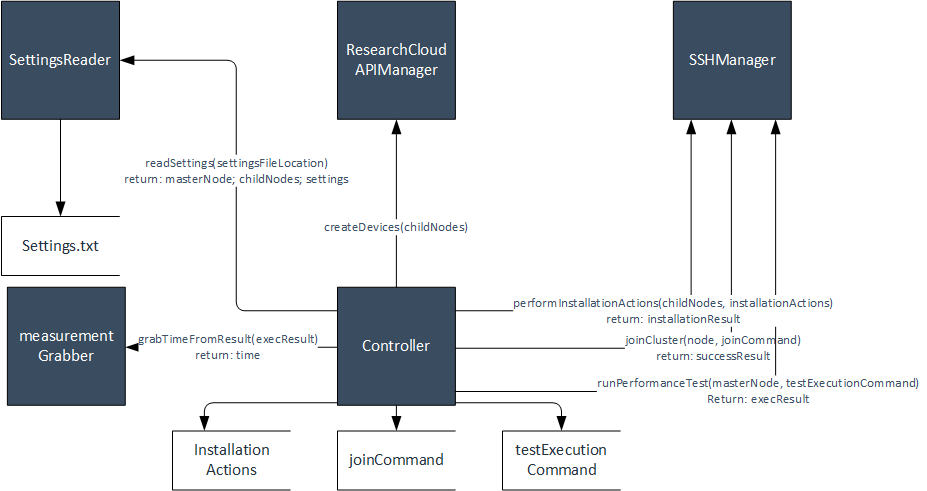
\includegraphics[width=\textwidth]{images/testing_software_components.png}

\textsuperscript{Figure 3.3.1 Testing software components}
\end{figure}

The second component is the SettingsReader. This component has the task to read out the settings file configured by the user and grabs all the necessary information out of it. In this file there has to be configured the settings for the master node and the test specifications on the one hand and the amount and specifications of the child nodes on the other hand. How this file could look like can be seen in Appendix B) Settings File for testing software.

The first five lines are for the masterNode. The first line is for the hostname, the second for the password, and the three following lines are for the Kubernetes join command. Thereby the first of those three lines is for the IP-Address and the other two lines are security keys to access the cluster. Those can be grabbed from the masterNode as described in chapter 3.1.

The next two lines are general settings. The first of them specifies how often a the test command should be executed per test specification to calculate a good average. The second line is for how many nodes should join the cluster after each test run.

After this there has to follow an empty line and then the configurations for the child nodes. Thereby, first has to be specified the hostname prefix, which the child nodes should get. They all need an individual name, which is the reason why there can be set a placeholder with ``<index>'', which is replaced by an increasing number. After that the amount of cores and the size of the memory can be specified. The last number stands for the amount of how many nodes of this configuration should be added. Any number of different worker node specifications can be added, but every specification of a worker node has to be split with an empty line.

The third component is an API Manager for the Research Cloud API. This provides all necessary functions for creating Cloud devices. How a JSON could look like, which is used for creating such a cloud device, can be seen in Appendix C) ResearchCloudAPI JSON. There need to be specified the hostname, the amount of CPUs, the memory, the operating system, the disk capacity and other configuration for the location of the datacenter, payments etc.

The fourth component is an SSH Manager, which offers the possibility to access cloud machines via SSH. This enables the possibility to install and configure everything necessary on the devices, add them to the cluster and run the tests on the master node. How this SSH Manager looks like can be seen in Appendix D) SSH Manager. It returns the prints of the executed commands, which is then used by the last component - the measurementGrabber.

This component grabs the time out of the result by a given scheme. These time data are then used to calculate an average out of all tests, which is then printed out for the user.

This architecture and the the first version of the project had been kept small because of insufficient time and for providing a easy-to-understand and clear project to present the possibility of automated testing. This influences several decisions which had to be made during the project.

The first decision was the environment, on which the project should be build on. Because the main part of Wildfire is build on Scala and so this language is pretty common in the project team, it has been decided to also build the testing software on Scala for offering a good insight for every team member on the one hand and for gaining experiences in this language on the other hand. This also offers the advantage of a quick and easy development of the main parts and a high amount of libraries and frameworks, because Scala is based on Java and can implement Java code. That's why this project was mainly written in Scala with some additions in Java.

A second decision was the structure of the settings file. One possibility was a structured and easy to read way with using XML or JSON. Another possibility was to use a simple txt file and read the needed informations line by line. Therefore the order of the information has to be determined in advance. But because of the insufficient time this way has been chosen for a faster way to implement the SettingsReader and to avoid additional libraries, which had to be used.

Another question was how to access the virtual Cloud devices via SSH. Therefore jcabi, a collection of small Java components, offers an SSH library, which enables access to other devices, execute commands and even return the answer of those devices.

A problem occurred while trying to access the Research Cloud API - because the creation based on previous build images, which could be an prepared device with all necessary installations, configurations and an created account for a unique possibility to access the devices, lasted longer than one day, this possibility was no option for quick, automated testing of different specifications. That forced to create blank devices instead and install everything up from the beginning for each device. Also the password had to be manually entered because for every device there is a random password created, which is no part of the returning JSON of the Research Cloud API. But this also solved the problem of fluctuating times the devices need to be created, after which the program could continue running. Because the user has to enter the password manually and is just able to do this after a successful creation, the program can wait for the user input of the password before continuing the following processes.

This leads to the sequence diagram shown in Appendix E) ``Testing software sequence diagram''.

First the user starts the program. Then the different kinds of settings - masterNode-Information, childNode-Configuration and other settings - are read out and written into appropriate datatypes. After it, the Controller forces the ResearchCloudAPIManager to create child nodes by a given list. Therefore it sends a request for every entry of the childNodesList. After a succesfull creation request for each of them and while the devices are creating the Controller waits for an input of the user with the passwords for every device. As soon as they are entered the programm adds the passwords to the appropriate device. After a password has been entered and added for every device the programm continues and the Controller uses the SSH Manager to perform all installation actions defined in a configurable txt file, which first has to be read out, for each of the childNodes.

Now the testing phase starts. For that the first nodes joins the cluster, a configurable amount of tests are run and for each test the time is measured. At the end of each test run the result of those tests is calculated and added to a list. Then the next test run starts and a configurable amount of nodes are added to the cluster. This is done by executing a command via the SSH Manager. After that the tests are run and the average time is calculated. This repeats over and over again until every node is connected and every test has been run. Last the list of all average times is printed out for the user.

These steps guarantee an almost fully automated testing with the only action the user has to take is to enter the passwords for the Cloud devices at the beginning. This enables faster and larger scaled tests and a good opportunity to compare the performance of Cloud machines with common, physical devices.
